\section{并行与并发}
Rust也同样支持常见的并行和并发操作,也同样分为进程,线程以及消息通信等等。

\subsection{线程}
Rust的线程操作必须使用闭包完成。在之前看到的闭包当中,通常采用的都是有参的闭包,
而在Rust的线程操作当中,则经常会遇到无参数的闭包;Rust的线程使用thread::spawn函数
进行实现:
\begin{code-block}{rust}
use std::thread;
use std::time::Duration;

fn main() {
    thread::spawn(|| {
        for i in 1..10 {
            println!("hi number {} from the spawned thread!", i);
            thread::sleep(Duration::from_millis(1));
        }
    });

    for i in 1..5 {
        println!("hi number {} from the main thread!", i);
        thread::sleep(Duration::from_millis(1));
    }
}
\end{code-block}
和其他语言的线程概念一样,当主线程结束时,所有的线程都会被终止。因此上述代码当中,
子线程(spawn)无法将所有的循环执行完成。为了达成所有进/线程执行完成之后才退出主
进/线程的目的,和其他的开发语言相同,需要在主进程当中调用join函数:
\begin{code-block}{rust}
fn main() {
    let handle = thread::spawn(|| {
        for i in 1..10 {
            println!("hi number {} from the spawned thread!", i);
            thread::sleep(Duration::from_millis(1));
        }
    });

    for i in 1..5 {
        println!("hi number {} from the main thread!", i);
        thread::sleep(Duration::from_millis(1));
    }
    handle.join().unwrap();
}
\end{code-block}
Thread::spawn的返回值是JoinHandle,是一个拥有所有权的值,当对其调用join方法时,
它会等待对应线程结束;而join的返回值是一个Result,可以按照之前介绍的方式进行处理。
同时,Join函数是一个阻塞式函数,只有当该函数运行结束之后,才会继续进行后续的操作。

多数情况下,Rust的线程不可能只会在内部运行,而和外部没有数据交互。但是,如果我们
直接使用外部数据,则会出现错误,比如下方的代码:
\begin{code-block}{rust}
fn main() {
    let v = vec![1, 2, 3];
    let handle = thread::spawn(|| {
        println!("Here's a vector: {:?}", v);
    });
    handle.join().unwrap();
}
\end{code-block}
\begin{figure}[H]
  \centering
  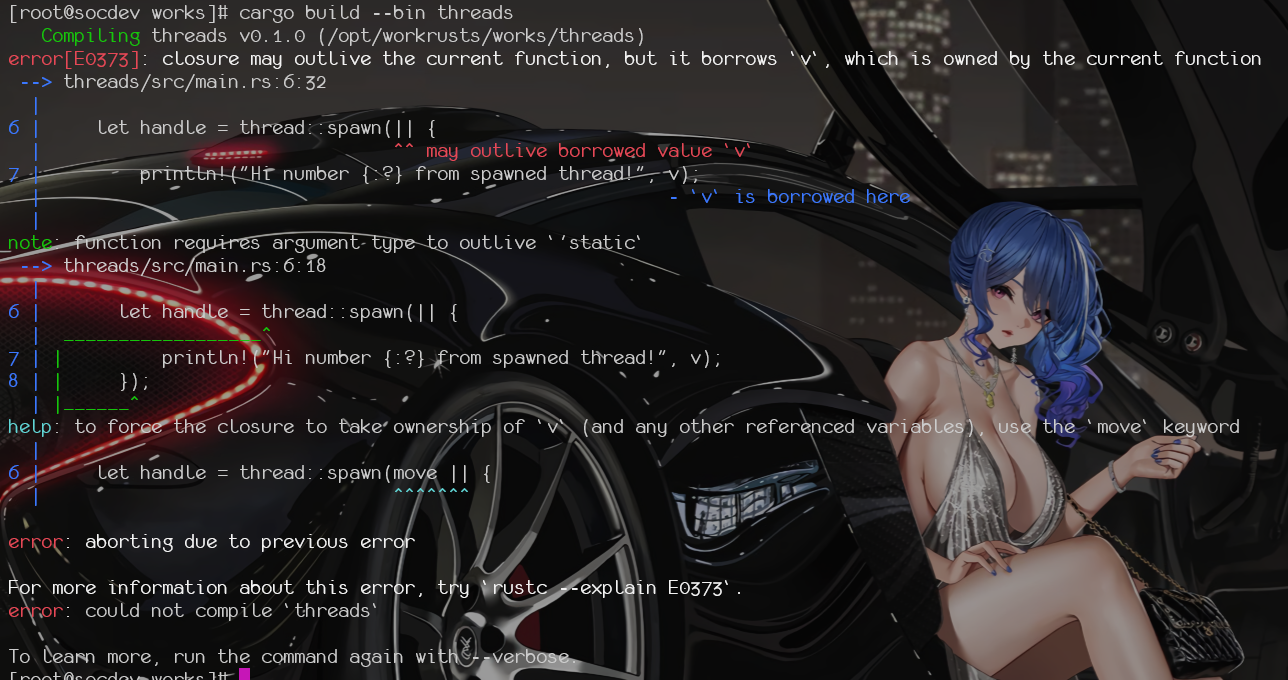
\includegraphics[width=\linewidth]{rust_thread_out_params.png}
  \caption{试图访问线程外部资源}
  \label{fig:rust_thread_out_params}
\end{figure}
线程使用的是闭包,从闭包的定义来说,是可以捕获并使用外部变量和数据的;但是,Rust
不知道这个线程到底会运行多长时间,因此无法知道对外部变量的引用是否一直有效,比如
下方的代码:
\begin{code-block}{rust}
fn main() {
    let v = vec![1, 2, 3];
    let handle = thread::spawn(|| {
        println!("Here's a vector: {:?}", v);
    });
    drop(v);
    handle.join().unwrap();
}
\end{code-block}
启动线程的同时,立即将v进行丢弃,线程内部无法知道v在运行阶段是否继续有效,就会
出现错误,因此,如果在线程当中使用默认的闭包模式,则无法对应的闭包是无法捕获以及
使用外部的变量和数据的。此时,则需要使用move闭包进行替换,即强制闭包获取外部变量
的所有权,而不是由Rust进行借用推断。但是需要注意,一旦使用move之后,在线程之外,
变量将无法再进行使用:
\begin{code-block}{rust}
fn main() {
    let v = vec![1, 2, 3];
    let handle = thread::spawn(move || {
        println!("Here's a vector: {:?}", v);
    });
    // 下方代码无法再进行执行
    // println!("{:?}", v);
    handle.join().unwrap();
}
\end{code-block}

\subsection{消息通信和消息传递}
每个线程做自己的事情,但是,不管什么编程语言,都需要考虑线程之间的数据交互问题。
Rust向Golang进行了学习,使用通信替换共享内存,来进行线程之间的数据传输。同样的,
Rust当中用于消息传递并发的主要工具是通道,该概念和Golang的通道概念相同。Rust的通道
分为2个角色:发送者和接收者,发送者发送消息,接收者接收消息,当发送者或者接收者任一
被丢弃时,则对应的通道被视为关闭。

Rust的通道采用mpsc::channel函数实现,mpsc表示多个生产者,单个消费者,因此,Rust
标准库实现通道的方式意味着一个通道可以有多个产生值的发送(sending)端,但只能有
一个消费这些值的接收(receiving)端。通道的实现示例如下:
\begin{code-block}{rust}
use std::sync::mpsc;
fn main() {
    let (sender, recevier) = mpsc::channel();
}
\end{code-block}
其中,函数的第一个返回值为发送者,第二个参数为接收者。使用通道发送数据通信的示例
如下:
\begin{code-block}{rust}
use std::sync::mpsc;
use std::thread;

fn main() {
    let (sender, recevier) = mpsc::channel();

    thread::spawn(move || {
        let val = "lucifer".to_string();
        match sender.send(val) {
            Ok(_) => println!("Send success"),
            Err(error) => println!("Send failed :{:?}", error),
        }
    });

    let res = match recevier.recv() {
        Ok(s) => s,
        Err(error) => {
            println!("Cannot recevie anything from sender: {:?}", error);
            "".to_string()
        }
    };
    println!("The result of channel is {}", res);
}
\end{code-block}
接收者接收消息有2种模式:默认的recv是阻塞式,返回一个Result<T, E>,当通道关闭时,
将返回Result当中的Error;而try\_recv是非阻塞式,同样是返回一个Result<T, E>,但是,
Result当中的Error表示没有接收到任何消息,可以使用for循环进行反复的尝试读取操作。
另外需要注意的是,Send函数会改变变量的所有权,当该函数执行之后,被发送的消息
(变量)将无法再使用。

但是,通道可以反复使用,而且和Golang的类似,Rust的通道也是可以进行迭代的,特别
是在接收消息时,通常采用for循环进行操作,减少了错误处理的代码,使得代码更具可读性:
\begin{code-block}{rust}
use std::sync::mpsc;
use std::thread;

fn main() {
    let (sender, recevier) = mpsc::channel();

    let handler = thread::spawn(move || {
        let vals = vec!["lucifer", "titans", "garuda"];
        for val in vals {
            match sender.send(val) {
                Ok(_) => println!("Send success"),
                Err(error) => println!("Send failed :{:?}", error),
            }
        }
    });

    for msg in recevier {
        println!("The msg is {}", msg);
    }

    match handler.join() {
        Err(error) => println!("Error{:?}", error),
        _ => (),
    }
}
\end{code-block}

同样的,由于Rust的通道默认是多生产者/单消费者,因此,可以通过多个发送端向单个接
收端发送消息。实际使用当中的多个发送端,则通常是某个发送端的克隆对象,如下:
\begin{code-block}{rust}
use std::sync::mpsc;
use std::thread;

fn main() {
    let (sender, recevier) = mpsc::channel();
    let sender_copy = sender.clone();

    let handler = thread::spawn(move || {
        let vals = vec!["lucifer", "titans", "garuda"];
        for val in vals {
            match sender.send(val) {
                Ok(_) => println!("Send success"),
                Err(error) => println!("Send failed :{:?}", error),
            }
        }
    });

    let handler_copy = thread::spawn(move || {
        let vals = vec!["zhangjl", "luoyan", "zhangzz"];
        for val in vals {
            match sender_copy.send(val) {
                Err(error) => println!("Send failed :{:?}", error),
                _ => (),
            }
        }
    });

    for msg in recevier {
        println!("The msg is {}", msg);
    }

    match handler_copy.join() {
        Err(error) => println!("Error{:?}", error),
        _ => (),
    }

    match handler.join() {
        Err(error) => println!("Error{:?}", error),
        _ => (),
    }
}
\end{code-block}

\subsection{共享状态}
在其他语言当中,有些特殊的场景,还是必须使用原有的线程并发概念——锁——来进行资源的
访问/读写控制。Rust当中同样存在锁,比较常见的就是互斥锁(互斥器,Mutex)以及原子
计数器(Arc)。在基本的操作上,互斥锁的使用和其他语言当中没有太大的区别:
\begin{code-block}{rust}
use std::sync::Mutex;
fn main() {
    let m = Mutex::new(5);
    {
        let mut num = m.lock().unwrap();
        *num = 6;
    }
    println!("m = {:?}", m);
}
\end{code-block}
注意,上述代码如果将内部大括号去除,则运行结束之后,m的状态还是锁定状态;但是,
有大括号,则表示大括号内部的段是一个有效的生命周期,当该生命周期结束之后,互斥
锁将自动释放。一旦获取了锁,就可以将返回值(在这里是num)视为一个其内部数据的
\underline{\color{red} \textbf{可变引用}}。类型系统确保了我们在使用m中的值之前
获取锁:Mutex<i32>并不是一个i32,所以必须获取锁才能使用这个i32值。

实质上,Mutex是一个智能指针,lock调用返回一个叫做MutexGuard的智能指针。这个智能
指针实现了Deref来指向其内部数据;同时也提供了一个Drop实现,使得MutexGuard离开作
用域时自动释放锁,即锁的释放是自动发生的。

但是默认情况下,Mutex是无法用于进行线程间的数据共享,如下:
\begin{code-block}{rust}
use std::rc::Rc;
use std::sync::Mutex;
use std::thread;

fn main() {
    let counter = Rc::new(Mutex::new(0));
    let mut handles = vec![];

    for _ in 0..10 {
        let counter = Rc::clone(&counter);
        let handle = thread::spawn(move || {
            let mut num = counter.lock().unwrap();

            *num += 1;
        });
        handles.push(handle);
    }

    for handle in handles {
        handle.join().unwrap();
    }

    println!("Result: {}", *counter.lock().unwrap());
}
\end{code-block}
上述代码会出现下面的类似错误:
\begin{figure}[H]
  \centering
  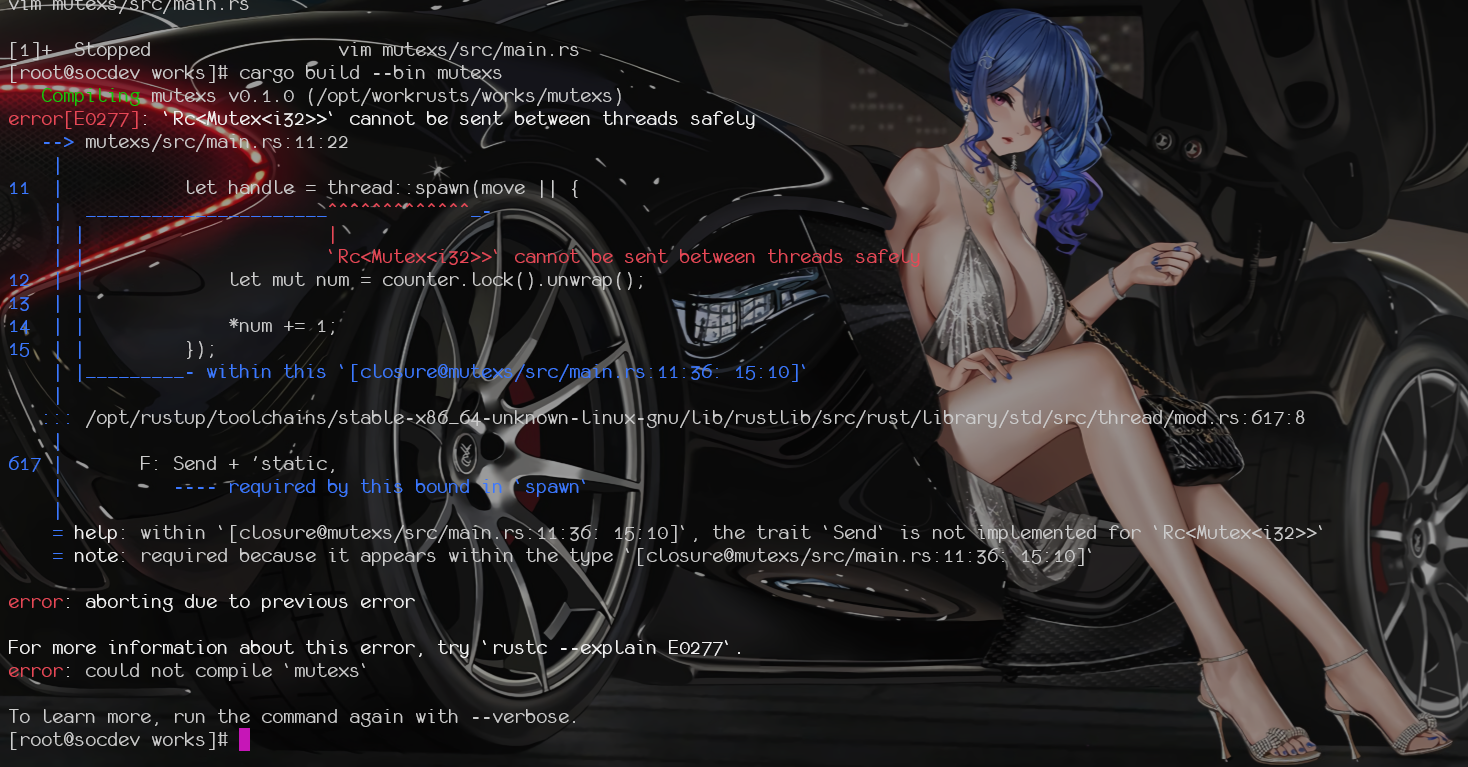
\includegraphics[scale=0.215]{rust_mutex_share_error.png}
  \caption{试图通过Rc共享Mutex的数据}
  \label{fig:rust_mutex_share_error}
\end{figure}
即之前提到的,Rc类型只能用于单线程/单进程环境。

而共享引用计数则需要使用Arc,它是可以安全的用于并发环境的类型,即原子引用计数,
可以在线程间进行共享所有权。Arc和Rc有相同的API,基本使用方法上类似。所有,可以直
接对上述代码进行修改:
\begin{code-block}{rust}
use std::sync::{Arc, Mutex};
use std::thread;
fn main() {
    let counter = Arc::new(Mutex::new(0));
    let mut handles = vec![];
    for _ in 0..10 {
        let counter = Arc::clone(&counter);
        let handle = thread::spawn(move || {
            let mut num = counter.lock().unwrap();
            *num += 1;
        });
        handles.push(handle);
    }
    for handle in handles {
        handle.join().unwrap();
    }
    println!("Result: {}", *counter.lock().unwrap());
}
\end{code-block}
通过这样简单的修改,成功实现了10个进程当中对同一个数值进行加法操作的功能。

\section{Match与模式匹配}
Match是Rust常用的语法糖,其用法不局限于之前所讲的范围。关于match的用法,还有很多,
并且,多数和模式匹配有关,接下来可以看一些常见的match和模式匹配的使用方式。
\begin{outline}[enumerate]
\1 多种匹配模式

在match表达式当中,可以用|匹配多个模式,表示或运算:
\begin{code-in-enumerate}{rust}
let x = 1;
match x {
    1 | 2 => println!("one or two"),
    3 => println!("three"),
    _ => println!("anything"),
}
\end{code-in-enumerate}

\1 使用..=匹配范围

..=语法允许匹配一个数值范围内的任意数据,常用于数值和字符:
\begin{code-in-enumerate}{rust}
let x = 5;
match x {
    1..=5 => println!("one through five"),
    _ => println!("something else"),
}

let y = 'c';
match y {
    'a'..='j' => println!("early ASCII letter"),
    'k'..='z' => println!("late ASCII letter"),
    _ => println!("something else"),
}
\end{code-in-enumerate}

\1 解构结构体

Let模式可以将结构体当中的字段/元素进行解构,单独或者批量赋予其他元素:
\begin{code-in-enumerate}{rust}
struct Point {
    x: i32,
    y: i32,
}
fn main() {
    let p = Point { x: 0, y: 7 };
    // 将p的x字段的值赋予a,y字段的值赋予b,a和b是整数类型,不是引用
    let Point { x: a, y: b } = p;
    // let Point {x: ref a, y: ref b} = p; 和上面类似,但是a和b是整数类型的引用
    // let Point {x: a, y: _} = p; 表示只需要将x的值赋予a,但不需要对y进行解构
    assert_eq!(0, a);
    assert_eq!(7, b);
    // let Point {x, y} = p; 将p的x字段的值赋予变量x,y字段的值赋予变量y
}
\end{code-in-enumerate}

\1 解构枚举类型

Match本身就是应枚举而生的,因此天然的可以使用它对枚举进行解构:
\begin{code-in-enumerate}{rust}
enum Message {
    Quit,
    Move { x: i32, y: i32 },
    Write(String),
    ChangeColor(i32, i32, i32),
}

fn main() {
    let msg = Message::ChangeColor(0, 160, 255);

    match msg {
        Message::Quit => {
            println!("The Quit variant has no data to destructure.")
        }
        Message::Move { x, y } => {
            println!("Move in the x direction {} and in the y direction {}", x, y);
        }
        Message::Write(text) => println!("Text message: {}", text),
        Message::ChangeColor(r, g, b) => {
            println!("Change the color to red {}, green {}, and blue {}", r, g, b)
        }
    }
}
\end{code-in-enumerate}

同样的,如果枚举当中嵌套了枚举,仍然可以使用match进行解构:
\begin{code-in-enumerate}{rust}
enum Color {
    Rgb(i32, i32, i32),
    Hsv(i32, i32, i32),
}

enum Message {
    Quit,
    Move { x: i32, y: i32 },
    Write(String),
    ChangeColor(Color),
}

fn main() {
    let msg = Message::ChangeColor(Color::Hsv(0, 160, 255));

    match msg {
        Message::ChangeColor(Color::Rgb(r, g, b)) => {
            println!("Change the color to red {}, green {}, and blue {}", r, g, b)
        }
        Message::ChangeColor(Color::Hsv(h, s, v)) => {
            println!(
                "Change the color to hue {}, saturation {}, and value {}",
                h, s, v
            )
        }
        _ => (),
    }
}
\end{code-in-enumerate}

\1 解构复合数据

用复杂的方式来混合、匹配和嵌套解构模式,解析出我们感兴趣的数据:
\begin{code-in-enumerate}{rust}
let ((feet, inches), Point {x, y}) = ((3, 10), Point { x: 3, y: -10 });
\end{code-in-enumerate}

\1 忽略不需要的元素

在Rust的当中,默认可以使用\_对不必要的变量进行忽略,通常用在match的最后分支,但是,
实际上也可以用去其他任意的模式,甚至是函数参数:
\begin{code-in-enumerate}{rust}
// 需要传入2个参数,但是忽略第一个参数
fn foo(_: i32, y: i32) {
    println!("This code only uses the y parameter: {}", y);
}

fn main() {
    foo(3, 4);
}
\end{code-in-enumerate}

除了使用\_进行忽略之外,还可以使用..语法糖进行忽略,但是针对结构体和元组存在区别:
结构体当中,忽略的是没有被列出的字段;而元组忽略的则是范围:
\begin{code-in-enumerate}{rust}
struct Point {
    x: i32,
    y: i32,
    z: i32,
}

fn main() {
    let origin = Point { x: 0, y: 0, z: 0 };
    // 将point的y进行忽略
    match origin {
        Point { x,z, .. } => println!("x is {}, z is {}", x, z),
    }

    let numbers = (2, 4, 8, 16, 32);
    match numbers {
        // 忽略元组当中除第1、2和最后一项的所有元素
        (first, second, .., last) => {
            println!("Some numbers: {}, {}, {}, ", first, second, last);
        }
    }
}
\end{code-in-enumerate}

\1 @绑定

运算符@允许我们在创建一个存放值的变量的同时测试其值是否匹配模式,比如测试字段是
否位于指定范围内,同时也希望能将其值绑定到另外的变量中以便此分支相关联的代码可以
使用它:
\begin{code-in-enumerate}{rust}
enum Message {
    Hello { id: i32 },
}

let msg = Message::Hello { id: 5 };

match msg {
    // 将变量id保存到另一个变量ip_variable当中
    Message::Hello { id: id_variable @ 3..=7 } => {
        println!("Found an id in range: {}", id_variable)
    },
    Message::Hello { id: 10..=12 } => {
        println!("Found an id in another range")
    },
    Message::Hello { id } => {
        println!("Found some other id: {}", id)
    },
}
\end{code-in-enumerate}


\end{outline}
